\documentclass[../zhang_thesis.tex]{subfiles}
\begin{document}

\chapter{Methodology}

%%%%%%%%%%%%%%%%%%%%%%%%%%%%%%%%%%%%%%%%%%%%%%%%%%%%%%%%%%%%%%%

\section{Battery Model}

As discussed in the previous section, this thesis considers the electrical-circuit battery model proposed by Chen and Rinc\'on-Mora~\cite{chen06} and shown in \autoref{fig:batt_model}. The left portion of the circuit models the capacity, SOC, and runtime, while the right portion models the transient i-v characteristics.  For convenience, the model is designed so that the SOC of the battery equals the voltage $V_\text{SOC}$, in volts. The parameters $C_\text{cap}$ and
$R_{sd}$ are assumed constant for a given battery and determine the capacity and self-discharge rate of the battery. The other parameters are all nonlinear functions of $V_\text{SOC}$ and determine the transient i-v response as well as the open-circuit voltage $V_\text{OC}$. From a typical TCL PL-383562 polymer lithium-ion battery, Chen and Rinc\'on-Mora extracted these parameters and fit them to curves, obtaining
\begin{gather}
    R_s(V_\text{SOC}) = 0.1562 e^{-24.37 V_\text{SOC}} + 0.07446 \label{eq:nl_param_1} \\
    R_{ts}(V_\text{SOC}) = 0.3208 e^{-29.14 V_\text{SOC}} + 0.04669 \\
    C_{ts}(V_\text{SOC}) = -752.9 e^{-13.51 V_\text{SOC}} + 703.6 \\
    R_{tl}(V_\text{SOC}) = 6.603 e^{-155.2 V_\text{SOC}} + 0.04984 \\
    C_{tl}(V_\text{SOC}) = -6056 e^{-27.12 V_\text{SOC}} + 4475 \\
    V_\text{OC}(V_\text{SOC}) = -1.031 e^{-35 V_\text{SOC}} + 3.685 + 0.2156 V_\text{SOC} - 0.1178 V_\text{SOC}^2 + 0.3201 V_\text{SOC}^3 \label{eq:nl_param_6}
\end{gather}
The resistance and capacitance parameters shown above are approximately constant for $\text{SOC}>0.2$ and change exponentially for $\text{SOC}<0.2$. The open-circuit voltage also changes exponentially for $\text{SOC}<0.2$ but is approximately linear for $\text{SOC}>0.2$. Note that the capacitances $C_{ts}$ and $C_{tl}$ are negative for SOC values close to zero, which is both unrealistic according to the experimental data collected by Chen and Rin\'on-Mora and problematic
mathematically. To solve this, a lower bound was placed on the $V_\text{SOC}$ input to the capacitance functions. Thus, for inputs below some threshold value $v_T$, the capacitances are adjusted to their value at that threshold, producing
\begin{align}
    \hat{C}_{ts}(V_\text{SOC}) &= \begin{cases}
        C_{ts}(V_\text{SOC}), & V_\text{SOC} \ge v_T \\
        C_{ts}(v_T), & V_\text{SOC} < v_T
        \end{cases} \label{eq:Cts_thres} \\
    \hat{C}_{tl}(V_\text{SOC}) &= \begin{cases}
        C_{tl}(V_\text{SOC}), & V_\text{SOC} \ge v_T \\
        C_{tl}(v_T), & V_\text{SOC} < v_T \label{eq:Ctl_thres}
        \end{cases}
\end{align}
The threshold $v_T$ was chosen based on the experimental data of Chen and Rin\'on-Mora, specifically so that the threshold capacitance values are approximately equal to the lowest such values measured by them. A threshold of $v_T=0.015$~V accomplishes this goal.

\begin{figure}[ht]
\psfrag{i}[][]{$i_\text{cell}$}
\psfrag{v}[][]{$V_\text{cell}$}
\psfrag{+}[][]{$+$}
\psfrag{-}[][]{$-$}
\psfrag{R}[][]{$R_{sd}$}
\psfrag{Vs}[][]{$V_\text{SOC}$}
\psfrag{C}[][]{$C_\text{cap}$}
\psfrag{Vo}[][]{$V_\text{OC}$}
\psfrag{Vc}[][]{$V_\text{cell}$}
\psfrag{Rs}[][]{$R_s$}
\psfrag{Ra}[][]{$R_{ts}$}
\psfrag{Ca}[][]{$C_{ts}$}
\psfrag{Va}[][]{$V_{ts}$}
\psfrag{Rb}[][]{$R_{tl}$}
\psfrag{Cb}[][]{$C_{tl}$}
\psfrag{Vb}[][]{$V_{tl}$}

\centering
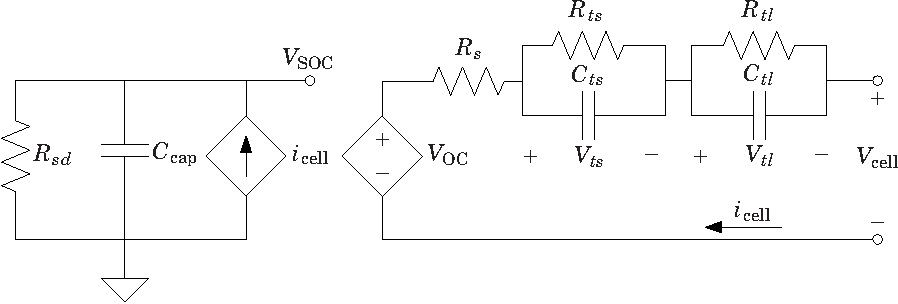
\includegraphics[width=\columnwidth]{batt_model}
\caption{Electrical-circuit battery model.}
\label{fig:batt_model}
\end{figure}

This study used the nonlinear parameters given by Chen and Rinc\'on-Mora for the implementation of a battery using their battery model in Matlab. In addition, the thresholding defined in \autorefs{eq:Cts_thres} and \ref{eq:Ctl_thres} was used with $v_T=0.015$~V. The other, constant parameters were chosen to produce a capacity of 1~Ah and a self-discharge rate of 4\% per month. To do so, the capacitance $C_\text{cap}$ is calculated to hold the desired capacity
when $V_\text{SOC}=1$~V, and then the resistance $R_{sd}$ is set to produce the desired self-discharge rate. For a given capacity of $C^\dag$ in Ah, $C_\text{cap}$ needs to be
\begin{equation}
    C_\text{cap} = \frac{Q}{V_\text{SOC}} = \frac{C^\dag}{1~\text{V}} = 3600 C^\dag \,[\text{F}].
\end{equation}
Then, the resistance $R_{sd}$ is chosen so that the time constant $\tau=RC$ results in the desired drop of $\xi=0.04$ over $T=1$~month as follows
\begin{gather}
    V(t) = V_0 e^{-T/\tau} = V_0 (1-\xi) \\
    \tau = -T/\ln(1-\xi) = -2592000/\ln 0.96 \,[\text{s}].
\end{gather}
Then, $R_{sd}=\tau/C_\text{cap}$. Thus, the parameters are $C_\text{cap}=3600$~F and $R_{sd}=17.6376~\mathrm{k}\Omega$.

In order to simulate the use of the modeled battery, discharging and charging loads were implemented, as shown in \autorefs{fig:batt_loads}. For discharging, a resistive load $R_L$ is placed across the battery terminals, creating a discharge rate of $i_\text{cell}=V_\text{cell}/R_L$. For charging, a negative resistance $-R_L$, where $R_L>0$, is used, creating a charging current of $-i_\text{cell}=V_\text{cell}/R_L$. Thus, any arbitrary charging or discharging current can be set
by choosing the appropriate resistance $R_L$. Furthermore, an open circuit can be simulated by choosing $R_L$ sufficiently large so that $i_\text{cell}\approx 0$. Additional consideration has to be taken to produce constant current and constant voltage charging conditions for standard charging procedure. Typically, the specific battery modeled by the given parameters is charged at a rate of $C_5/5$ until a terminal voltage of $4.2$~V is reached, where $C_5/5$ is the discharge
rate at which a full battery is completely discharged in 5 hours. Then, the battery is charged at a constant voltage of $4.2$~V until the charging current is below $C_5/20$. The constant current condition is met by varying $R_L$ so that $V_\text{cell}/R_L$ stays constant, while the constant voltage condition is met by varying $R_L$ so that $i_\text{cell} R_L$ stays constant.

\begin{figure}[ht]
\centering
\begin{subfigure}[c]{0.4\textwidth}
    \psfrag{i}[][]{$i_\text{cell}$}
\psfrag{v}[][]{$V_\text{cell}$}
\psfrag{+}[][]{$+$}
\psfrag{-}[][]{$-$}
\psfrag{R}[][]{$R_L$}

\centering
%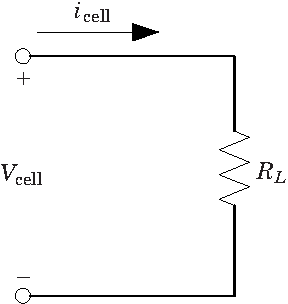
\includegraphics[width=0.75\columnwidth]{resistive_load}

\end{subfigure}
\begin{subfigure}[c]{0.55\textwidth}
    \psfrag{i}[][]{$i_\text{cell}$}
\psfrag{v}[][]{$V_\text{cell}$}
\psfrag{y}[][]{$V_o$}
\psfrag{+}[][]{$+$}
\psfrag{-}[][]{$-$}
\psfrag{R}[][]{$\lvert R_L \rvert$}
\psfrag{Ra}[][]{$R_1$}
\psfrag{Rb}[][]{$R_1$}

\centering
%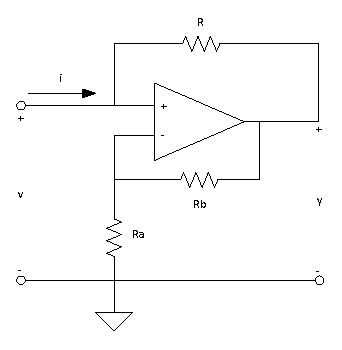
\includegraphics[width=0.9\columnwidth]{nrc}

\end{subfigure}
\caption{Loads to (a) discharge and (b) charge the battery.}
\label{fig:batt_loads}
\end{figure}

This use of the load $R_L$ to control the current $i_\text{cell}$ suggests that it is the input to the system. Moreover, the outputs of the system are $V_\text{cell}$ and $i_\text{cell}$. However, since knowledge of one of them along with $R_L$ allows for the calculation of the other, the two outputs have a known relationship between them. Therefore, only one of the outputs is necessary to fully define the input-output relationship of the system. In this study, the voltage
$V_\text{cell}$ was chosen as the output.

For ease of numerical simulation, it is useful to find the state-space system for the circuit. The state-space representation is derived using the physical variable definition, in which
the state variables are chosen to represent the voltages across the capacitors. Choosing $x_1=V_\text{SOC}$, $x_2=V_{ts}$, and $x_3=V_{tl}$ achieves this goal and results in the state-space representation
\begin{align}
    \dot{x}_1 &= - \frac{x_1}{R_{sd}C_\text{cap}} - \frac{V_\text{OC}(x_1)-x_2-x_3}{(R_s(x_1)+R_L)C_\text{cap}} + f_{w,1}(\mathbf{x},R_L,\mathbf{w}) \\
    \dot{x}_2 &= - \frac{x_2}{R_{ts}(x_1)C_{ts}(x_1)} + \frac{V_\text{OC}(x_1) - x_2 - x_3}{(R_s(x_1)+R_L)C_{ts}(x_1)} + f_{w,2}(\mathbf{x},R_L,\mathbf{w}) \\
    \dot{x}_3 &= - \frac{x_3}{R_{tl}(x_1)C_{tl}(x_1)} + \frac{V_\text{OC}(x_1) - x_2 - x_3}{(R_s(x_1)+R_L)C_{tl}(x_1)} + f_{w,3}(\mathbf{x},R_L,\mathbf{w}) \\
%    \dot{x}_2 &= - \frac{x_2}{R_{ts}(x_1) C_{ts}(x_1)} + \frac{i_{cell}}{C_{ts}(x_1)} \\
%    \dot{x}_3 &= - \frac{x_3}{R_{tl}(x_1) C_{tl}(x_1)} + \frac{i_{cell}}{C_{tl}(x_1)} \\
    V_\text{cell} &= \frac{V_\text{OC}(x_1) - x_2 - x_3}{1+R_s(x_1)/R_L} + f_v(\mathbf{x},R_L,\mathbf{v}),
\end{align}
where $R_L$ is the input to the system, $V_\text{cell}$ is the output, $f_w$ is the process noise function, $f_v$ is the measurement noise function, and the nonlinear parameters depending on $x_1$ are given by \autorefs{eq:nl_param_1} through \ref{eq:nl_param_6} along with the thresholding defined in \autorefs{eq:Cts_thres} and \ref{eq:Ctl_thres}. It is obvious from this formulation that the system is nonlinear to both the input and the states. In order to establish the noise expressions, the types of
noise present in the battery have to first be determined.

This thesis assumes that the process and measurement noises in this system are due to thermal noise in the resistances for the internal impedance of the battery $R_s$, $R_{ts}$, and $R_{tl}$, and for the load $R_L$. This is motivated by measurements of the voltage noise in batteries conducted by Boggs et al.\ that showed the measured noise is mainly due to thermal noise; the correlation between the battery terminals suppresses shot noise~\cite{boggs95}. This thermal noise is assumed to
be Gaussian white noise with a power spectral density (PSD) of~\cite{stremler82}
\begin{equation}
    S_n(\omega) \cong 2kT\ \text{watts per Hz} \qquad \text{for} \qquad |\omega| \ll 2\pi kT/h,
\end{equation}
where $T$ is the temperature of the conducting medium in Kelvin, $k$ is the Boltzmann's constant, and $h$ is the Planck's constant. \autoref{fig:batt_noisy} shows that the thermal noise due to the resistances is modeled as voltage sources in series with the resistances, with PSDs of $S_v(\omega)=2kTR$ for a corresponding resistance $R$. Using this definition, the noise functions are given by
\begin{align}
    f_{w,1} &= \frac{v_{n_s}+v_{n_L}}{(R_s(x_1)+R_L)C_\text{cap}} \\
    f_{w,2} &= \frac{v_{n_{ts}}}{R_{ts}(x_1)C_{ts}(x_1)} - \frac{v_{n_s}+v_{n_L}}{(R_s(x_1)+R_L)C_{ts}(x_1)} \\
    f_{w,3} &= \frac{v_{n_{tl}}}{R_{tl}(x_1)C_{tl}(x_1)} - \frac{v_{n_s}+v_{n_L}}{(R_s(x_1)+R_L)C_{tl}(x_1)} \\
    f_v &= - \frac{v_{n_s}+v_{n_L}}{1+R_s(x_1)/R_L}.
\end{align}
It can be seen that the resistances change over time, which causes the covariance of the sources $v_n$ to also change. For the purposes of modeling, it is useful to define noise variables that have constant covariance. Using the square root of the power supplied by the noise sources as the noise variables accomplishes this goal and produces the variables $w_1=v_{n_s}/\sqrt{R_s}$, $w_2=v_{n_{ts}}/\sqrt{R_{ts}}$, $w_3=v_{n_{tl}}/\sqrt{R_{tl}}$, and $w_4=v_{n_L}/\sqrt{R_L}$, which all have
constant covariances of $2kT$. Then, the state space representation of the system becomes
\begin{align}
    \dot{x}_1 &= - \frac{x_1}{R_{sd}C_\text{cap}} - \frac{V_\text{OC}(x_1) - x_2 - x_3 - \sqrt{R_s(x_1)}w_1 - \sqrt{R_L}w_4}{(R_s(x_1)+R_L)C_\text{cap}} \\
    \dot{x}_2 &= - \frac{x_2 - \sqrt{R_{ts}(x_1)}w_2}{R_{ts}(x_1)C_{ts}(x_1)} + \frac{V_\text{OC}(x_1) - x_2 - x_3 - \sqrt{R_s(x_1)}w_1 - \sqrt{R_L}w_4}{(R_s(x_1)+R_L)C_{ts}(x_1)} \\
    \dot{x}_3 &= - \frac{x_3 - \sqrt{R_{tl}(x_1)}w_3}{R_{tl}(x_1)C_{tl}(x_1)} + \frac{V_\text{OC}(x_1) - x_2 - x_3 - \sqrt{R_s(x_1)}w_1 - \sqrt{R_L}w_4}{(R_s(x_1)+R_L)C_{tl}(x_1)} \\
    V_\text{cell} &= \frac{V_\text{OC}(x_1) - x_2 - x_3 - \sqrt{R_s(x_1)}w_1 - \sqrt{R_L}w_4}{1+R_s(x_1)/R_L}.
\end{align}
This thesis assumed that a standard temperature of $T=290$~Kelvin. Therefore, the noise variables have covariances of $\sigma^2=2kT=8.0078\times 10^{-21}$~W/Hz.

\begin{figure}[ht]
\psfrag{i}[][]{$i_\text{cell}$}
\psfrag{v}[][]{$V_\text{cell}$}
\psfrag{+}[][]{$+$}
\psfrag{-}[][]{$-$}
\psfrag{Vo}[][]{$V_\text{OC}$}
\psfrag{Vc}[][]{$V_\text{cell}$}
\psfrag{Rs}[][]{$R_s$}
\psfrag{Ra}[][]{$R_{ts}$}
\psfrag{Ca}[][]{$C_{ts}$}
\psfrag{Va}[][]{$V_{ts}$}
\psfrag{Rb}[][]{$R_{tl}$}
\psfrag{Cb}[][]{$C_{tl}$}
\psfrag{Vb}[][]{$V_{tl}$}
\psfrag{RL}[][]{$R_L$}
\psfrag{vns}[][]{$v_{n_s}$}
\psfrag{vts}[][]{$v_{n_{ts}}$}
\psfrag{vtl}[][]{$v_{n_{tl}}$}
\psfrag{vnl}[][]{$v_{n_L}$}

\centering
%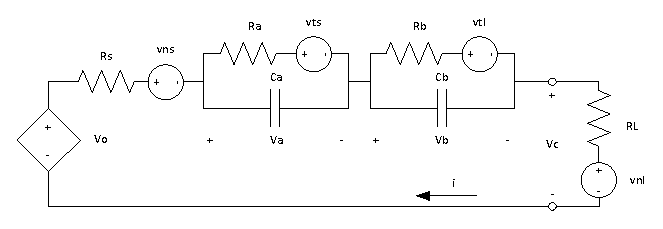
\includegraphics[width=\columnwidth]{batt_noisy}

\caption{Modeling of thermal noise in resistances as voltage sources in series with the resistances.}
\label{fig:batt_noisy}
\end{figure}

\section{Simulation Setup}

In order to generate the input and output of the system, the battery model was implemented in Simulink. \autoref{fig:batt_load_exp} shows a simulation of the battery, assuming no noise, discharged with $R_L=5~\Omega$ from 5 to 120 minutes and charged with $R_L=-5~\Omega$ from 150 to 250 minutes. A mechanism was implemented that bounded the SOC to $0\le\text{SOC}\le 1$, which can be seen in $i_\text{cell}$. \autoref{fig:batt_load_exp_noisy} shows a simulation with the same input, assuming
thermal noise. It can be seen that the effect of noise is minimal. This is better seen in \autoref{fig:batt_noise_comp}, which shows the squared difference between the outputs of the noiseless and noisy systems.

\begin{figure}[ht]
\centering
% This file is generated by the MATLAB m-file laprint.m. It can be included
% into LaTeX documents using the packages graphicx, color and psfrag.
% It is accompanied by a postscript file. A sample LaTeX file is:
%    \documentclass{article}\usepackage{graphicx,color,psfrag}
%    \begin{document}% This file is generated by the MATLAB m-file laprint.m. It can be included
% into LaTeX documents using the packages graphicx, color and psfrag.
% It is accompanied by a postscript file. A sample LaTeX file is:
%    \documentclass{article}\usepackage{graphicx,color,psfrag}
%    \begin{document}% This file is generated by the MATLAB m-file laprint.m. It can be included
% into LaTeX documents using the packages graphicx, color and psfrag.
% It is accompanied by a postscript file. A sample LaTeX file is:
%    \documentclass{article}\usepackage{graphicx,color,psfrag}
%    \begin{document}\input{batt_load_exp}\end{document}
% See http://www.mathworks.de/matlabcentral/fileexchange/loadFile.do?objectId=4638
% for recent versions of laprint.m.
%
% created by:           LaPrint version 3.16 (13.9.2004)
% created on:           18-Feb-2014 21:34:20
% eps bounding box:     15 cm x 8.1771 cm
% comment:              
%
\begin{psfrags}%
\psfragscanon%
%
% text strings:
\psfrag{s05}[t][t]{\color[rgb]{0,0,0}\setlength{\tabcolsep}{0pt}\begin{tabular}{c}Time (seconds)\end{tabular}}%
\psfrag{s06}[b][b]{\color[rgb]{0,0,0}\setlength{\tabcolsep}{0pt}\begin{tabular}{c}$\mathrm{V_{cell}}$\end{tabular}}%
\psfrag{s07}[b][b]{\color[rgb]{0,0,0}\setlength{\tabcolsep}{0pt}\begin{tabular}{c}Time Series Plot:$\mathrm{V_{cell}}$\end{tabular}}%
\psfrag{s08}[t][t]{\color[rgb]{0,0,0}\setlength{\tabcolsep}{0pt}\begin{tabular}{c}Time (seconds)\end{tabular}}%
\psfrag{s09}[b][b]{\color[rgb]{0,0,0}\setlength{\tabcolsep}{0pt}\begin{tabular}{c}$\mathrm{i_{cell}}$\end{tabular}}%
\psfrag{s10}[b][b]{\color[rgb]{0,0,0}\setlength{\tabcolsep}{0pt}\begin{tabular}{c}Time Series Plot:$\mathrm{i_{cell}}$\end{tabular}}%
\psfrag{s11}[t][t]{\color[rgb]{0,0,0}\setlength{\tabcolsep}{0pt}\begin{tabular}{c}Time (seconds)\end{tabular}}%
\psfrag{s12}[b][b]{\color[rgb]{0,0,0}\setlength{\tabcolsep}{0pt}\begin{tabular}{c}$R_L$\end{tabular}}%
%
% xticklabels:
\psfrag{x01}[t][t]{0}%
\psfrag{x02}[t][t]{5000}%
\psfrag{x03}[t][t]{10000}%
\psfrag{x04}[t][t]{15000}%
\psfrag{x05}[t][t]{0}%
\psfrag{x06}[t][t]{5000}%
\psfrag{x07}[t][t]{10000}%
\psfrag{x08}[t][t]{15000}%
\psfrag{x09}[t][t]{0}%
\psfrag{x10}[t][t]{5000}%
\psfrag{x11}[t][t]{10000}%
\psfrag{x12}[t][t]{15000}%
%
% yticklabels:
\psfrag{v01}[r][r]{-6}%
\psfrag{v02}[r][r]{-4}%
\psfrag{v03}[r][r]{-2}%
\psfrag{v04}[r][r]{0}%
\psfrag{v05}[r][r]{2}%
\psfrag{v06}[r][r]{4}%
\psfrag{v07}[r][r]{6}%
\psfrag{v08}[r][r]{-1}%
\psfrag{v09}[r][r]{-0.5}%
\psfrag{v10}[r][r]{0}%
\psfrag{v11}[r][r]{0.5}%
\psfrag{v12}[r][r]{1}%
\psfrag{v13}[r][r]{2}%
\psfrag{v14}[r][r]{2.5}%
\psfrag{v15}[r][r]{3}%
\psfrag{v16}[r][r]{3.5}%
\psfrag{v17}[r][r]{4}%
\psfrag{v18}[r][r]{4.5}%
%
% Figure:
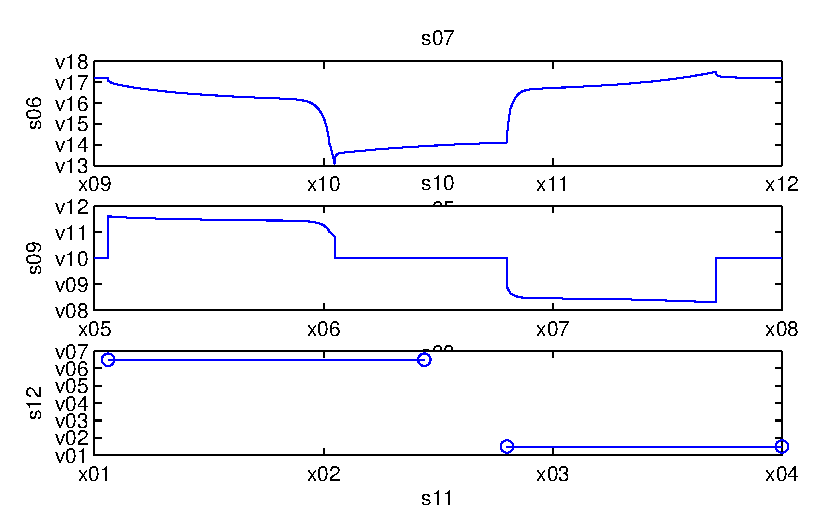
\includegraphics[width=12cm]{batt_load_exp.eps}%
\end{psfrags}%
%
% End batt_load_exp.tex
\end{document}
% See http://www.mathworks.de/matlabcentral/fileexchange/loadFile.do?objectId=4638
% for recent versions of laprint.m.
%
% created by:           LaPrint version 3.16 (13.9.2004)
% created on:           18-Feb-2014 21:34:20
% eps bounding box:     15 cm x 8.1771 cm
% comment:              
%
\begin{psfrags}%
\psfragscanon%
%
% text strings:
\psfrag{s05}[t][t]{\color[rgb]{0,0,0}\setlength{\tabcolsep}{0pt}\begin{tabular}{c}Time (seconds)\end{tabular}}%
\psfrag{s06}[b][b]{\color[rgb]{0,0,0}\setlength{\tabcolsep}{0pt}\begin{tabular}{c}$\mathrm{V_{cell}}$\end{tabular}}%
\psfrag{s07}[b][b]{\color[rgb]{0,0,0}\setlength{\tabcolsep}{0pt}\begin{tabular}{c}Time Series Plot:$\mathrm{V_{cell}}$\end{tabular}}%
\psfrag{s08}[t][t]{\color[rgb]{0,0,0}\setlength{\tabcolsep}{0pt}\begin{tabular}{c}Time (seconds)\end{tabular}}%
\psfrag{s09}[b][b]{\color[rgb]{0,0,0}\setlength{\tabcolsep}{0pt}\begin{tabular}{c}$\mathrm{i_{cell}}$\end{tabular}}%
\psfrag{s10}[b][b]{\color[rgb]{0,0,0}\setlength{\tabcolsep}{0pt}\begin{tabular}{c}Time Series Plot:$\mathrm{i_{cell}}$\end{tabular}}%
\psfrag{s11}[t][t]{\color[rgb]{0,0,0}\setlength{\tabcolsep}{0pt}\begin{tabular}{c}Time (seconds)\end{tabular}}%
\psfrag{s12}[b][b]{\color[rgb]{0,0,0}\setlength{\tabcolsep}{0pt}\begin{tabular}{c}$R_L$\end{tabular}}%
%
% xticklabels:
\psfrag{x01}[t][t]{0}%
\psfrag{x02}[t][t]{5000}%
\psfrag{x03}[t][t]{10000}%
\psfrag{x04}[t][t]{15000}%
\psfrag{x05}[t][t]{0}%
\psfrag{x06}[t][t]{5000}%
\psfrag{x07}[t][t]{10000}%
\psfrag{x08}[t][t]{15000}%
\psfrag{x09}[t][t]{0}%
\psfrag{x10}[t][t]{5000}%
\psfrag{x11}[t][t]{10000}%
\psfrag{x12}[t][t]{15000}%
%
% yticklabels:
\psfrag{v01}[r][r]{-6}%
\psfrag{v02}[r][r]{-4}%
\psfrag{v03}[r][r]{-2}%
\psfrag{v04}[r][r]{0}%
\psfrag{v05}[r][r]{2}%
\psfrag{v06}[r][r]{4}%
\psfrag{v07}[r][r]{6}%
\psfrag{v08}[r][r]{-1}%
\psfrag{v09}[r][r]{-0.5}%
\psfrag{v10}[r][r]{0}%
\psfrag{v11}[r][r]{0.5}%
\psfrag{v12}[r][r]{1}%
\psfrag{v13}[r][r]{2}%
\psfrag{v14}[r][r]{2.5}%
\psfrag{v15}[r][r]{3}%
\psfrag{v16}[r][r]{3.5}%
\psfrag{v17}[r][r]{4}%
\psfrag{v18}[r][r]{4.5}%
%
% Figure:
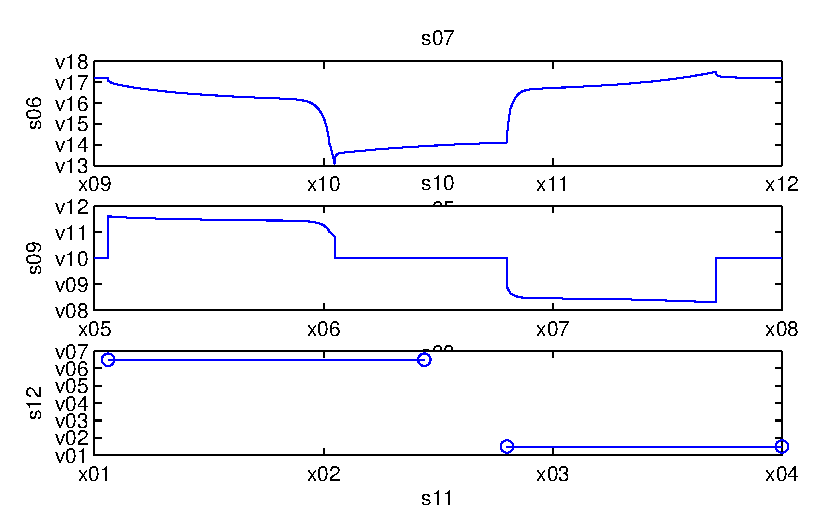
\includegraphics[width=12cm]{batt_load_exp.eps}%
\end{psfrags}%
%
% End batt_load_exp.tex
\end{document}
% See http://www.mathworks.de/matlabcentral/fileexchange/loadFile.do?objectId=4638
% for recent versions of laprint.m.
%
% created by:           LaPrint version 3.16 (13.9.2004)
% created on:           18-Feb-2014 21:34:20
% eps bounding box:     15 cm x 8.1771 cm
% comment:              
%
\begin{psfrags}%
\psfragscanon%
%
% text strings:
\psfrag{s05}[t][t]{\color[rgb]{0,0,0}\setlength{\tabcolsep}{0pt}\begin{tabular}{c}Time (seconds)\end{tabular}}%
\psfrag{s06}[b][b]{\color[rgb]{0,0,0}\setlength{\tabcolsep}{0pt}\begin{tabular}{c}$\mathrm{V_{cell}}$\end{tabular}}%
\psfrag{s07}[b][b]{\color[rgb]{0,0,0}\setlength{\tabcolsep}{0pt}\begin{tabular}{c}Time Series Plot:$\mathrm{V_{cell}}$\end{tabular}}%
\psfrag{s08}[t][t]{\color[rgb]{0,0,0}\setlength{\tabcolsep}{0pt}\begin{tabular}{c}Time (seconds)\end{tabular}}%
\psfrag{s09}[b][b]{\color[rgb]{0,0,0}\setlength{\tabcolsep}{0pt}\begin{tabular}{c}$\mathrm{i_{cell}}$\end{tabular}}%
\psfrag{s10}[b][b]{\color[rgb]{0,0,0}\setlength{\tabcolsep}{0pt}\begin{tabular}{c}Time Series Plot:$\mathrm{i_{cell}}$\end{tabular}}%
\psfrag{s11}[t][t]{\color[rgb]{0,0,0}\setlength{\tabcolsep}{0pt}\begin{tabular}{c}Time (seconds)\end{tabular}}%
\psfrag{s12}[b][b]{\color[rgb]{0,0,0}\setlength{\tabcolsep}{0pt}\begin{tabular}{c}$R_L$\end{tabular}}%
%
% xticklabels:
\psfrag{x01}[t][t]{0}%
\psfrag{x02}[t][t]{5000}%
\psfrag{x03}[t][t]{10000}%
\psfrag{x04}[t][t]{15000}%
\psfrag{x05}[t][t]{0}%
\psfrag{x06}[t][t]{5000}%
\psfrag{x07}[t][t]{10000}%
\psfrag{x08}[t][t]{15000}%
\psfrag{x09}[t][t]{0}%
\psfrag{x10}[t][t]{5000}%
\psfrag{x11}[t][t]{10000}%
\psfrag{x12}[t][t]{15000}%
%
% yticklabels:
\psfrag{v01}[r][r]{-6}%
\psfrag{v02}[r][r]{-4}%
\psfrag{v03}[r][r]{-2}%
\psfrag{v04}[r][r]{0}%
\psfrag{v05}[r][r]{2}%
\psfrag{v06}[r][r]{4}%
\psfrag{v07}[r][r]{6}%
\psfrag{v08}[r][r]{-1}%
\psfrag{v09}[r][r]{-0.5}%
\psfrag{v10}[r][r]{0}%
\psfrag{v11}[r][r]{0.5}%
\psfrag{v12}[r][r]{1}%
\psfrag{v13}[r][r]{2}%
\psfrag{v14}[r][r]{2.5}%
\psfrag{v15}[r][r]{3}%
\psfrag{v16}[r][r]{3.5}%
\psfrag{v17}[r][r]{4}%
\psfrag{v18}[r][r]{4.5}%
%
% Figure:
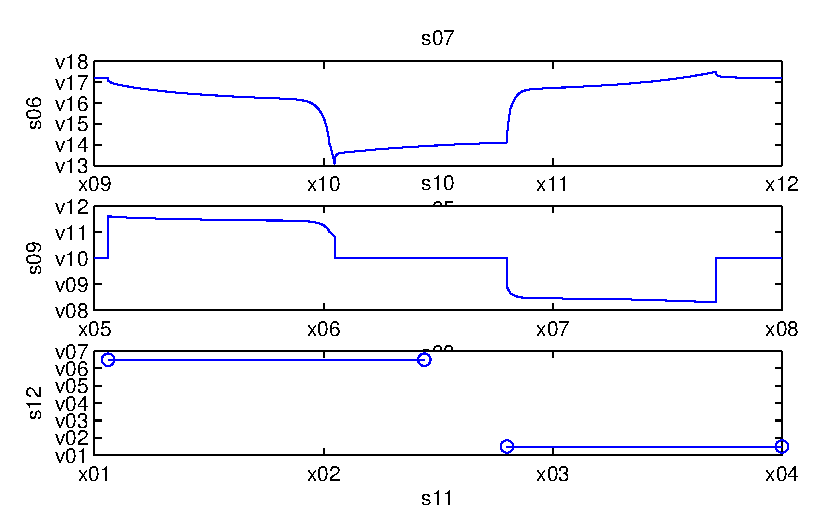
\includegraphics[width=12cm]{batt_load_exp.eps}%
\end{psfrags}%
%
% End batt_load_exp.tex

\caption{Test of discharging battery with resistive load and charging using negative resistance assuming no noise.}
\label{fig:batt_load_exp}
\end{figure}

\begin{figure}[ht]
\centering
% This file is generated by the MATLAB m-file laprint.m. It can be included
% into LaTeX documents using the packages graphicx, color and psfrag.
% It is accompanied by a postscript file. A sample LaTeX file is:
%    \documentclass{article}\usepackage{graphicx,color,psfrag}
%    \begin{document}% This file is generated by the MATLAB m-file laprint.m. It can be included
% into LaTeX documents using the packages graphicx, color and psfrag.
% It is accompanied by a postscript file. A sample LaTeX file is:
%    \documentclass{article}\usepackage{graphicx,color,psfrag}
%    \begin{document}% This file is generated by the MATLAB m-file laprint.m. It can be included
% into LaTeX documents using the packages graphicx, color and psfrag.
% It is accompanied by a postscript file. A sample LaTeX file is:
%    \documentclass{article}\usepackage{graphicx,color,psfrag}
%    \begin{document}\input{batt_load_exp_noisy}\end{document}
% See http://www.mathworks.de/matlabcentral/fileexchange/loadFile.do?objectId=4638
% for recent versions of laprint.m.
%
% created by:           LaPrint version 3.16 (13.9.2004)
% created on:           21-Feb-2014 19:38:25
% eps bounding box:     15 cm x 8.1771 cm
% comment:              
%
\begin{psfrags}%
\psfragscanon%
%
% text strings:
\psfrag{s05}[t][t]{\color[rgb]{0,0,0}\setlength{\tabcolsep}{0pt}\begin{tabular}{c}\end{tabular}}%
\psfrag{s06}[b][b]{\color[rgb]{0,0,0}\setlength{\tabcolsep}{0pt}\begin{tabular}{c}$V_\text{cell}$\end{tabular}}%
\psfrag{s08}[t][t]{\color[rgb]{0,0,0}\setlength{\tabcolsep}{0pt}\begin{tabular}{c}\end{tabular}}%
\psfrag{s09}[b][b]{\color[rgb]{0,0,0}\setlength{\tabcolsep}{0pt}\begin{tabular}{c}$i_\text{cell}$\end{tabular}}%
\psfrag{s11}[t][t]{\color[rgb]{0,0,0}\setlength{\tabcolsep}{0pt}\begin{tabular}{c}Time (seconds)\end{tabular}}%
\psfrag{s12}[b][b]{\color[rgb]{0,0,0}\setlength{\tabcolsep}{0pt}\begin{tabular}{c}$R_L$\end{tabular}}%
%
% xticklabels:
\psfrag{x01}[t][t]{0}%
\psfrag{x02}[t][t]{5000}%
\psfrag{x03}[t][t]{10000}%
\psfrag{x04}[t][t]{15000}%
\psfrag{x05}[t][t]{0}%
\psfrag{x06}[t][t]{5000}%
\psfrag{x07}[t][t]{10000}%
\psfrag{x08}[t][t]{15000}%
\psfrag{x09}[t][t]{0}%
\psfrag{x10}[t][t]{5000}%
\psfrag{x11}[t][t]{10000}%
\psfrag{x12}[t][t]{15000}%
%
% yticklabels:
\psfrag{v01}[r][r]{-6}%
\psfrag{v02}[r][r]{-4}%
\psfrag{v03}[r][r]{-2}%
\psfrag{v04}[r][r]{0}%
\psfrag{v05}[r][r]{2}%
\psfrag{v06}[r][r]{4}%
\psfrag{v07}[r][r]{6}%
\psfrag{v08}[r][r]{-1}%
\psfrag{v09}[r][r]{-0.5}%
\psfrag{v10}[r][r]{0}%
\psfrag{v11}[r][r]{0.5}%
\psfrag{v12}[r][r]{1}%
\psfrag{v13}[r][r]{2}%
\psfrag{v14}[r][r]{2.5}%
\psfrag{v15}[r][r]{3}%
\psfrag{v16}[r][r]{3.5}%
\psfrag{v17}[r][r]{4}%
\psfrag{v18}[r][r]{4.5}%
%
% Figure:
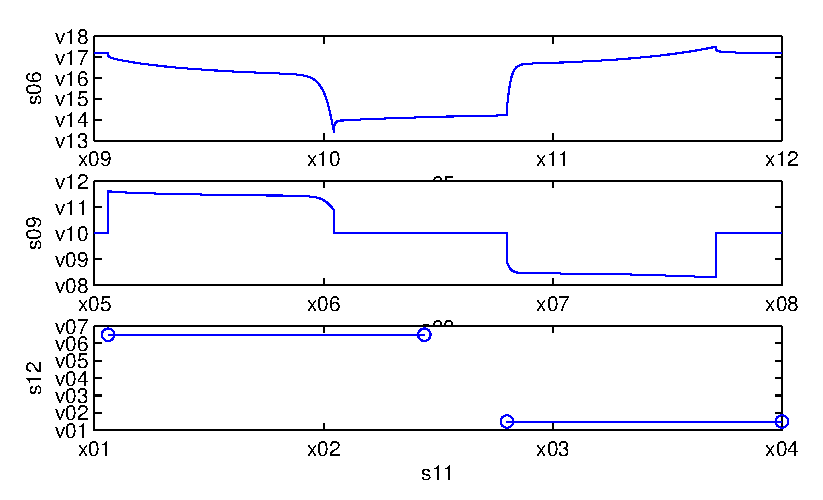
\includegraphics[width=15cm]{batt_load_exp_noisy.eps}%
\end{psfrags}%
%
% End batt_load_exp_noisy.tex
\end{document}
% See http://www.mathworks.de/matlabcentral/fileexchange/loadFile.do?objectId=4638
% for recent versions of laprint.m.
%
% created by:           LaPrint version 3.16 (13.9.2004)
% created on:           21-Feb-2014 19:38:25
% eps bounding box:     15 cm x 8.1771 cm
% comment:              
%
\begin{psfrags}%
\psfragscanon%
%
% text strings:
\psfrag{s05}[t][t]{\color[rgb]{0,0,0}\setlength{\tabcolsep}{0pt}\begin{tabular}{c}\end{tabular}}%
\psfrag{s06}[b][b]{\color[rgb]{0,0,0}\setlength{\tabcolsep}{0pt}\begin{tabular}{c}$V_\text{cell}$\end{tabular}}%
\psfrag{s08}[t][t]{\color[rgb]{0,0,0}\setlength{\tabcolsep}{0pt}\begin{tabular}{c}\end{tabular}}%
\psfrag{s09}[b][b]{\color[rgb]{0,0,0}\setlength{\tabcolsep}{0pt}\begin{tabular}{c}$i_\text{cell}$\end{tabular}}%
\psfrag{s11}[t][t]{\color[rgb]{0,0,0}\setlength{\tabcolsep}{0pt}\begin{tabular}{c}Time (seconds)\end{tabular}}%
\psfrag{s12}[b][b]{\color[rgb]{0,0,0}\setlength{\tabcolsep}{0pt}\begin{tabular}{c}$R_L$\end{tabular}}%
%
% xticklabels:
\psfrag{x01}[t][t]{0}%
\psfrag{x02}[t][t]{5000}%
\psfrag{x03}[t][t]{10000}%
\psfrag{x04}[t][t]{15000}%
\psfrag{x05}[t][t]{0}%
\psfrag{x06}[t][t]{5000}%
\psfrag{x07}[t][t]{10000}%
\psfrag{x08}[t][t]{15000}%
\psfrag{x09}[t][t]{0}%
\psfrag{x10}[t][t]{5000}%
\psfrag{x11}[t][t]{10000}%
\psfrag{x12}[t][t]{15000}%
%
% yticklabels:
\psfrag{v01}[r][r]{-6}%
\psfrag{v02}[r][r]{-4}%
\psfrag{v03}[r][r]{-2}%
\psfrag{v04}[r][r]{0}%
\psfrag{v05}[r][r]{2}%
\psfrag{v06}[r][r]{4}%
\psfrag{v07}[r][r]{6}%
\psfrag{v08}[r][r]{-1}%
\psfrag{v09}[r][r]{-0.5}%
\psfrag{v10}[r][r]{0}%
\psfrag{v11}[r][r]{0.5}%
\psfrag{v12}[r][r]{1}%
\psfrag{v13}[r][r]{2}%
\psfrag{v14}[r][r]{2.5}%
\psfrag{v15}[r][r]{3}%
\psfrag{v16}[r][r]{3.5}%
\psfrag{v17}[r][r]{4}%
\psfrag{v18}[r][r]{4.5}%
%
% Figure:
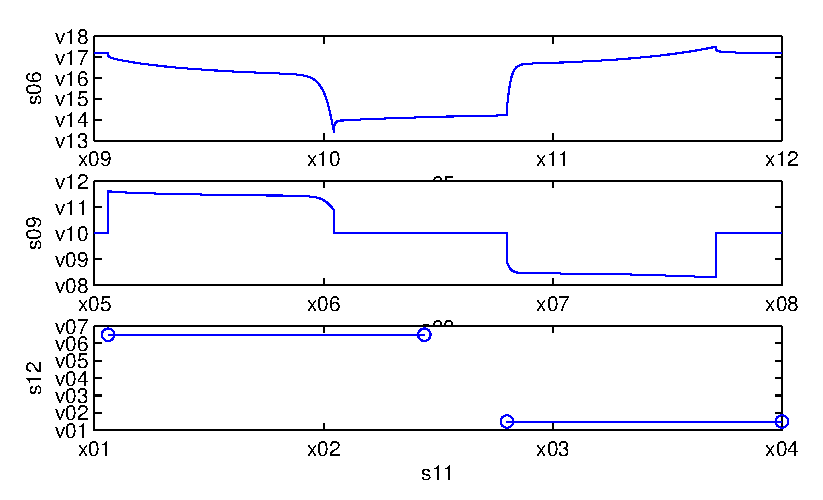
\includegraphics[width=15cm]{batt_load_exp_noisy.eps}%
\end{psfrags}%
%
% End batt_load_exp_noisy.tex
\end{document}
% See http://www.mathworks.de/matlabcentral/fileexchange/loadFile.do?objectId=4638
% for recent versions of laprint.m.
%
% created by:           LaPrint version 3.16 (13.9.2004)
% created on:           21-Feb-2014 19:38:25
% eps bounding box:     15 cm x 8.1771 cm
% comment:              
%
\begin{psfrags}%
\psfragscanon%
%
% text strings:
\psfrag{s05}[t][t]{\color[rgb]{0,0,0}\setlength{\tabcolsep}{0pt}\begin{tabular}{c}\end{tabular}}%
\psfrag{s06}[b][b]{\color[rgb]{0,0,0}\setlength{\tabcolsep}{0pt}\begin{tabular}{c}$V_\text{cell}$\end{tabular}}%
\psfrag{s08}[t][t]{\color[rgb]{0,0,0}\setlength{\tabcolsep}{0pt}\begin{tabular}{c}\end{tabular}}%
\psfrag{s09}[b][b]{\color[rgb]{0,0,0}\setlength{\tabcolsep}{0pt}\begin{tabular}{c}$i_\text{cell}$\end{tabular}}%
\psfrag{s11}[t][t]{\color[rgb]{0,0,0}\setlength{\tabcolsep}{0pt}\begin{tabular}{c}Time (seconds)\end{tabular}}%
\psfrag{s12}[b][b]{\color[rgb]{0,0,0}\setlength{\tabcolsep}{0pt}\begin{tabular}{c}$R_L$\end{tabular}}%
%
% xticklabels:
\psfrag{x01}[t][t]{0}%
\psfrag{x02}[t][t]{5000}%
\psfrag{x03}[t][t]{10000}%
\psfrag{x04}[t][t]{15000}%
\psfrag{x05}[t][t]{0}%
\psfrag{x06}[t][t]{5000}%
\psfrag{x07}[t][t]{10000}%
\psfrag{x08}[t][t]{15000}%
\psfrag{x09}[t][t]{0}%
\psfrag{x10}[t][t]{5000}%
\psfrag{x11}[t][t]{10000}%
\psfrag{x12}[t][t]{15000}%
%
% yticklabels:
\psfrag{v01}[r][r]{-6}%
\psfrag{v02}[r][r]{-4}%
\psfrag{v03}[r][r]{-2}%
\psfrag{v04}[r][r]{0}%
\psfrag{v05}[r][r]{2}%
\psfrag{v06}[r][r]{4}%
\psfrag{v07}[r][r]{6}%
\psfrag{v08}[r][r]{-1}%
\psfrag{v09}[r][r]{-0.5}%
\psfrag{v10}[r][r]{0}%
\psfrag{v11}[r][r]{0.5}%
\psfrag{v12}[r][r]{1}%
\psfrag{v13}[r][r]{2}%
\psfrag{v14}[r][r]{2.5}%
\psfrag{v15}[r][r]{3}%
\psfrag{v16}[r][r]{3.5}%
\psfrag{v17}[r][r]{4}%
\psfrag{v18}[r][r]{4.5}%
%
% Figure:
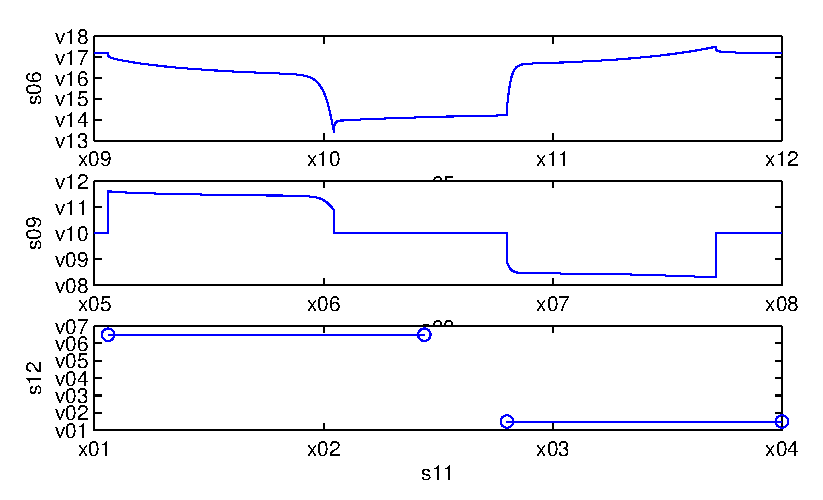
\includegraphics[width=15cm]{batt_load_exp_noisy.eps}%
\end{psfrags}%
%
% End batt_load_exp_noisy.tex

\caption{Test of discharging battery with resistive load and charging using negative resistance assuming thermal noise.}
\label{fig:batt_load_exp_noisy}
\end{figure}

\clearpage

\begin{figure}[ht]
\centering
% This file is generated by the MATLAB m-file laprint.m. It can be included
% into LaTeX documents using the packages graphicx, color and psfrag.
% It is accompanied by a postscript file. A sample LaTeX file is:
%    \documentclass{article}\usepackage{graphicx,color,psfrag}
%    \begin{document}% This file is generated by the MATLAB m-file laprint.m. It can be included
% into LaTeX documents using the packages graphicx, color and psfrag.
% It is accompanied by a postscript file. A sample LaTeX file is:
%    \documentclass{article}\usepackage{graphicx,color,psfrag}
%    \begin{document}% This file is generated by the MATLAB m-file laprint.m. It can be included
% into LaTeX documents using the packages graphicx, color and psfrag.
% It is accompanied by a postscript file. A sample LaTeX file is:
%    \documentclass{article}\usepackage{graphicx,color,psfrag}
%    \begin{document}\input{batt_noise_comp}\end{document}
% See http://www.mathworks.de/matlabcentral/fileexchange/loadFile.do?objectId=4638
% for recent versions of laprint.m.
%
% created by:           LaPrint version 3.16 (13.9.2004)
% created on:           25-Feb-2014 20:15:36
% eps bounding box:     15 cm x 11.25 cm
% comment:              
%
\begin{psfrags}%
\psfragscanon%
%
% text strings:
\psfrag{s09}[b][b]{\color[rgb]{0,0,0}\setlength{\tabcolsep}{0pt}\begin{tabular}{c}$V_\text{cell}$ MSE [dBW]\end{tabular}}%
\psfrag{s10}[b][b]{\color[rgb]{0,0,0}\setlength{\tabcolsep}{0pt}\begin{tabular}{c}$i_\text{cell}$ MSE [dBW]\end{tabular}}%
\psfrag{s11}[t][t]{\color[rgb]{0,0,0}\setlength{\tabcolsep}{0pt}\begin{tabular}{c}Time (seconds)\end{tabular}}%
\psfrag{s12}[b][b]{\color[rgb]{0,0,0}\setlength{\tabcolsep}{0pt}\begin{tabular}{c}$R_L$\end{tabular}}%
%
% xticklabels:
\psfrag{x01}[t][t]{0}%
\psfrag{x02}[t][t]{5000}%
\psfrag{x03}[t][t]{10000}%
\psfrag{x04}[t][t]{15000}%
\psfrag{x05}[t][t]{0}%
\psfrag{x06}[t][t]{5000}%
\psfrag{x07}[t][t]{10000}%
\psfrag{x08}[t][t]{15000}%
\psfrag{x09}[t][t]{0}%
\psfrag{x10}[t][t]{5000}%
\psfrag{x11}[t][t]{10000}%
\psfrag{x12}[t][t]{15000}%
%
% yticklabels:
\psfrag{v01}[r][r]{-5}%
\psfrag{v02}[r][r]{0}%
\psfrag{v03}[r][r]{5}%
\psfrag{v04}[r][r]{-400}%
\psfrag{v05}[r][r]{-200}%
\psfrag{v06}[r][r]{0}%
\psfrag{v07}[r][r]{-300}%
\psfrag{v08}[r][r]{-200}%
\psfrag{v09}[r][r]{-100}%
\psfrag{v10}[r][r]{0}%
%
% Figure:
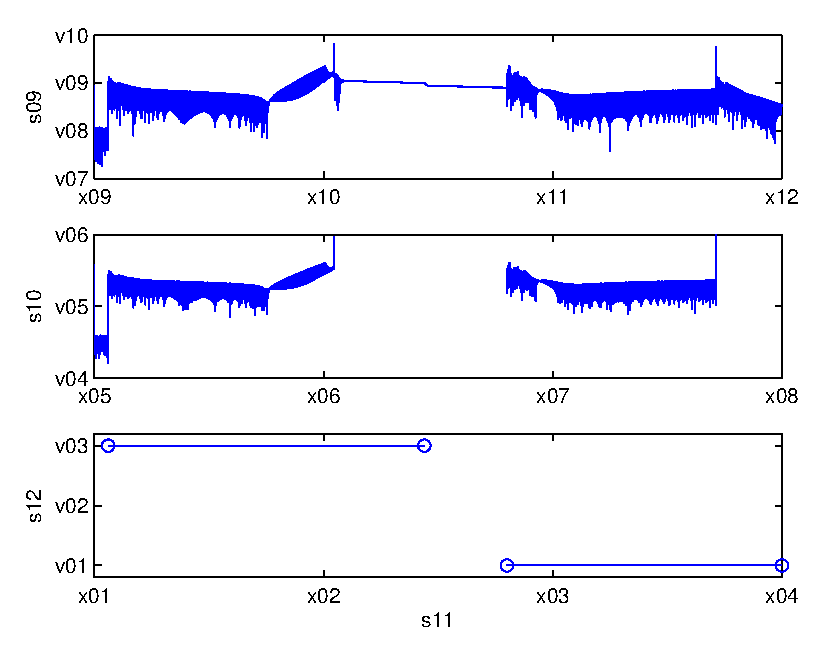
\includegraphics[width=15cm]{batt_noise_comp.eps}%
\end{psfrags}%
%
% End batt_noise_comp.tex
\end{document}
% See http://www.mathworks.de/matlabcentral/fileexchange/loadFile.do?objectId=4638
% for recent versions of laprint.m.
%
% created by:           LaPrint version 3.16 (13.9.2004)
% created on:           25-Feb-2014 20:15:36
% eps bounding box:     15 cm x 11.25 cm
% comment:              
%
\begin{psfrags}%
\psfragscanon%
%
% text strings:
\psfrag{s09}[b][b]{\color[rgb]{0,0,0}\setlength{\tabcolsep}{0pt}\begin{tabular}{c}$V_\text{cell}$ MSE [dBW]\end{tabular}}%
\psfrag{s10}[b][b]{\color[rgb]{0,0,0}\setlength{\tabcolsep}{0pt}\begin{tabular}{c}$i_\text{cell}$ MSE [dBW]\end{tabular}}%
\psfrag{s11}[t][t]{\color[rgb]{0,0,0}\setlength{\tabcolsep}{0pt}\begin{tabular}{c}Time (seconds)\end{tabular}}%
\psfrag{s12}[b][b]{\color[rgb]{0,0,0}\setlength{\tabcolsep}{0pt}\begin{tabular}{c}$R_L$\end{tabular}}%
%
% xticklabels:
\psfrag{x01}[t][t]{0}%
\psfrag{x02}[t][t]{5000}%
\psfrag{x03}[t][t]{10000}%
\psfrag{x04}[t][t]{15000}%
\psfrag{x05}[t][t]{0}%
\psfrag{x06}[t][t]{5000}%
\psfrag{x07}[t][t]{10000}%
\psfrag{x08}[t][t]{15000}%
\psfrag{x09}[t][t]{0}%
\psfrag{x10}[t][t]{5000}%
\psfrag{x11}[t][t]{10000}%
\psfrag{x12}[t][t]{15000}%
%
% yticklabels:
\psfrag{v01}[r][r]{-5}%
\psfrag{v02}[r][r]{0}%
\psfrag{v03}[r][r]{5}%
\psfrag{v04}[r][r]{-400}%
\psfrag{v05}[r][r]{-200}%
\psfrag{v06}[r][r]{0}%
\psfrag{v07}[r][r]{-300}%
\psfrag{v08}[r][r]{-200}%
\psfrag{v09}[r][r]{-100}%
\psfrag{v10}[r][r]{0}%
%
% Figure:
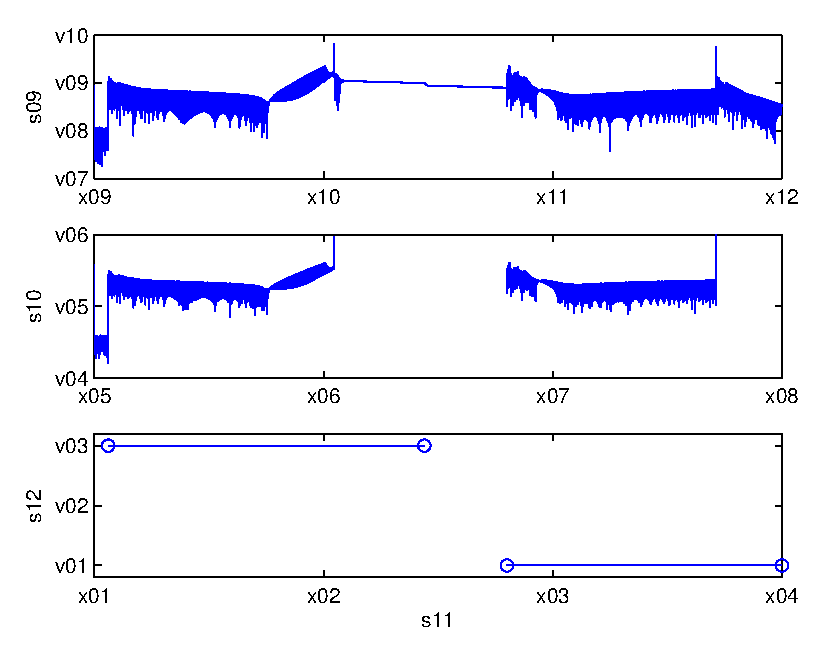
\includegraphics[width=15cm]{batt_noise_comp.eps}%
\end{psfrags}%
%
% End batt_noise_comp.tex
\end{document}
% See http://www.mathworks.de/matlabcentral/fileexchange/loadFile.do?objectId=4638
% for recent versions of laprint.m.
%
% created by:           LaPrint version 3.16 (13.9.2004)
% created on:           25-Feb-2014 20:15:36
% eps bounding box:     15 cm x 11.25 cm
% comment:              
%
\begin{psfrags}%
\psfragscanon%
%
% text strings:
\psfrag{s09}[b][b]{\color[rgb]{0,0,0}\setlength{\tabcolsep}{0pt}\begin{tabular}{c}$V_\text{cell}$ MSE [dBW]\end{tabular}}%
\psfrag{s10}[b][b]{\color[rgb]{0,0,0}\setlength{\tabcolsep}{0pt}\begin{tabular}{c}$i_\text{cell}$ MSE [dBW]\end{tabular}}%
\psfrag{s11}[t][t]{\color[rgb]{0,0,0}\setlength{\tabcolsep}{0pt}\begin{tabular}{c}Time (seconds)\end{tabular}}%
\psfrag{s12}[b][b]{\color[rgb]{0,0,0}\setlength{\tabcolsep}{0pt}\begin{tabular}{c}$R_L$\end{tabular}}%
%
% xticklabels:
\psfrag{x01}[t][t]{0}%
\psfrag{x02}[t][t]{5000}%
\psfrag{x03}[t][t]{10000}%
\psfrag{x04}[t][t]{15000}%
\psfrag{x05}[t][t]{0}%
\psfrag{x06}[t][t]{5000}%
\psfrag{x07}[t][t]{10000}%
\psfrag{x08}[t][t]{15000}%
\psfrag{x09}[t][t]{0}%
\psfrag{x10}[t][t]{5000}%
\psfrag{x11}[t][t]{10000}%
\psfrag{x12}[t][t]{15000}%
%
% yticklabels:
\psfrag{v01}[r][r]{-5}%
\psfrag{v02}[r][r]{0}%
\psfrag{v03}[r][r]{5}%
\psfrag{v04}[r][r]{-400}%
\psfrag{v05}[r][r]{-200}%
\psfrag{v06}[r][r]{0}%
\psfrag{v07}[r][r]{-300}%
\psfrag{v08}[r][r]{-200}%
\psfrag{v09}[r][r]{-100}%
\psfrag{v10}[r][r]{0}%
%
% Figure:
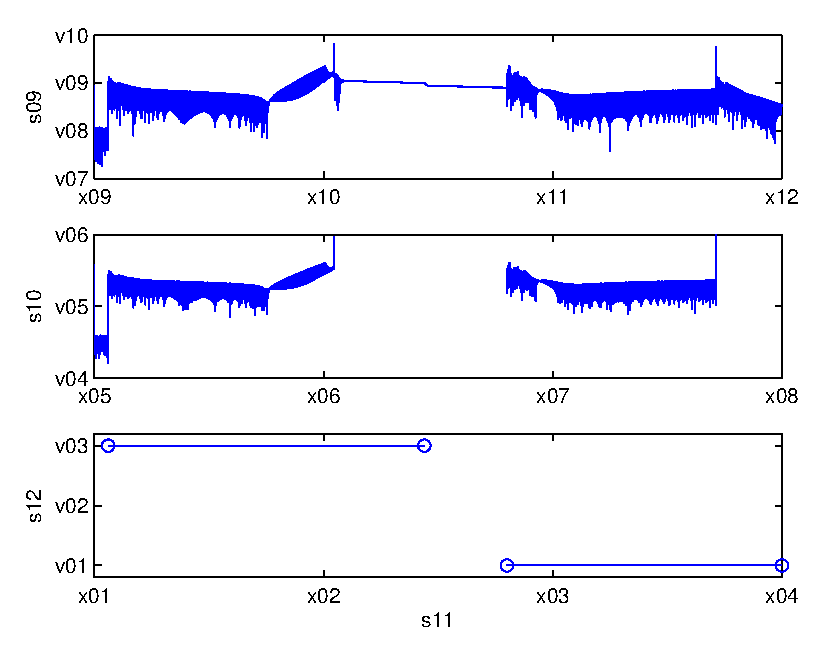
\includegraphics[width=15cm]{batt_noise_comp.eps}%
\end{psfrags}%
%
% End batt_noise_comp.tex

\caption{Comparison of outputs between noiseless and noisy systems.}
\label{fig:batt_noise_comp}
\end{figure}

\section{Filter Implementations}

%As was seen in the last section, the degree of nonlinearity of the battery model necessitates the use of a nonlinear filter. However, for SOC$>0.2$, the dynamics behave approximately linearly, because the resistance and capacitance parameters are approximately constant. Since the battery operates in this ``linear'' region for the majority of the time, it is useful to compare the performance of a linear filter to the nonlinear filters discussed in \autoref{sec:nl_filt}.

%In order to determine the necessity of incorporating the nonlinear relationship between $V_\text{SOC}$ and $V_\text{OC}$ in the filter design, the linearized right-hand circuit with $V_\text{SOC}=0.6$~V and the left-hand circuit were processed by a Kalman filter in each iteration and in that order, with the nonlinearity calculated implicitly.
% the left-hand circuit along with the right-hand circuit linearized at $V_\text{SOC}=0.6$~V were consecutively processed by the Kalman filter in each itera


\end{document}
